\documentclass[12pt,a4paper]{report}

\usepackage[utf8]{inputenc}
\usepackage{graphicx}
\usepackage{float}
\usepackage{caption}

\renewcommand{\labelitemi}{--}
\renewcommand{\texttt}[1]{{\normalfont #1}}

\makeatletter
\def\@makechapterhead#1{%
    \vspace*{20pt}%
    {\parindent \z@ \raggedright \normalfont
        \Huge\bfseries #1\par\nobreak
        \vskip 30pt}}
\def\@makeschapterhead#1{%
    \vspace*{20pt}%
    {\parindent \z@ \raggedright \normalfont
        \Huge\bfseries #1\par\nobreak
        \vskip 30pt}}
\makeatother

\newcommand{\placeholderbox}[2]{%
    \begin{center}
        \fbox{%
            \begin{minipage}[c][#2][c]{0.92\textwidth}
                \centering
                #1
            \end{minipage}
        }
    \end{center}
}

\begin{document}

\begin{titlepage}
    \centering
    \vspace*{2cm}

    {\Large Emanuele Sebastiano Reggiani\par}
    \vspace{2cm}

    {\Huge\bfseries Ricolorazione di immagini tramite Diffusion Models e 3D LUT\par}
    \vspace{1.5cm}

    {\large Relazione tecnica di progetto\par}
    \vfill

    {\large \today\par}
\end{titlepage}

\tableofcontents
\clearpage

\chapter{Descrizione del progetto}

Il progetto sviluppato ha come obiettivo la ricolorazione di immagini preservando il contenuto originale, la composizione e la geometria della scena. L'approccio implementato combina modelli di generazione image-to-image basati su \textit{Diffusion Models} con il fitting di una \textit{3D Look-Up Table} (3D LUT), in modo da separare la fase creativa di generazione cromatica dalla fase deterministica di applicazione della trasformazione colore.

La pipeline principale parte da un'immagine originale e produce una target image ricolorata tramite un backend diffusion, oppure utilizza una target image gia' disponibile. Successivamente vengono campionate coppie di pixel corrispondenti tra immagine originale e target, e tali coppie sono usate per stimare una 3D LUT. La LUT approssima la trasformazione cromatica osservata nella target e viene poi applicata all'immagine originale. In questo modo il risultato finale mantiene la struttura dell'immagine sorgente, mentre trasferisce il color grading ottenuto dal modello generativo.

\section{Componenti implementate}

Il codice e' organizzato come package Python e fornisce una command line interface chiamata \texttt{color-adjust}. I comandi principali implementati sono:

\begin{itemize}
    \item \texttt{grade}: genera una target cromatica deterministica, utile per verificare il comportamento della LUT senza introdurre variabilita' generativa;
    \item \texttt{diffuse}: genera una target image tramite HuggingFace Diffusers;
    \item \texttt{fit}: stima una 3D LUT a partire da immagine originale e target gia' disponibile;
    \item \texttt{refine}: fitta una LUT globale e applica una correzione residual locale tramite maschera morbida;
    \item \texttt{pipeline}: esegue l'intero flusso, dalla generazione della target al fitting della LUT e al salvataggio del risultato finale, con opzione \texttt{--refine} per attivare il passaggio residual;
    \item \texttt{apply}: applica una LUT salvata a una nuova immagine.
\end{itemize}

La parte diffusion supporta piu' backend. Per immagini di dimensione maggiore viene applicato un ridimensionamento controllato dal parametro \texttt{max-side}, cosi' da rendere la generazione piu' gestibile.

\section{Backend diffusion disponibili}

I backend diffusion sono definiti come preset, cioe' configurazioni che associano un model id, una pipeline Diffusers e un insieme di parametri predefiniti. L'obiettivo e' poter confrontare modelli diversi mantenendo la stessa interfaccia da command line.

\begin{table}[htbp]
    \centering
    \small
    \begin{tabular}{p{0.18\textwidth}p{0.28\textwidth}p{0.20\textwidth}p{0.24\textwidth}}
        \hline
        Backend & Modello & Pipeline & Parametri principali \\
        \hline
        \texttt{instruct-pix2pix} & \texttt{timbrooks/instruct-pix2pix} & InstructPix2Pix & IGS 1.2, 30 steps \\
        \texttt{img2img} & \texttt{runwayml/stable-diffusion-v1-5} & SD Img2Img & strength 0.25, CFG 7.5, 30 steps \\
        \texttt{sd15} & \texttt{runwayml/stable-diffusion-v1-5} & SD Img2Img & strength 0.55, CFG 8.0, 50 steps \\
        \texttt{sdxl} & \texttt{stabilityai/stable-diffusion-xl-base-1.0} & Auto Img2Img & strength 0.55, CFG 9.0, 50 steps \\
        \texttt{sdxl-turbo} & \texttt{stabilityai/sdxl-turbo} & Auto Img2Img & strength 0.75, CFG 0.0, 4 steps \\
        \hline
    \end{tabular}
    \caption{Backend diffusion disponibili nella pipeline.}
    \label{tab:backend-diffusion}
\end{table}

Il backend predefinito e' \texttt{instruct-pix2pix}. Questo modello e' basato sulla famiglia Stable Diffusion, ma e' specializzato per eseguire modifiche guidate da istruzioni testuali. A differenza di un normale workflow \texttt{img2img}, il prompt non deve descrivere l'intera immagine, ma puo' essere formulato come comando di editing, ad esempio ``make the image warmer'' oppure ``make the whole image more vibrant''. Il parametro specifico piu' importante e' \texttt{image-guidance-scale}, che controlla quanto il risultato deve restare vicino all'immagine di input.

Il backend \texttt{img2img} utilizza Stable Diffusion 1.5 in modalita' image-to-image con \texttt{strength} basso. Questa configurazione e' stata pensata per i test di ricolorazione perche' tende a preservare meglio composizione e oggetti, lasciando comunque al prompt la possibilita' di modificare il color grading. Il backend \texttt{sd15} usa lo stesso modello, ma con parametri piu' aggressivi: una \texttt{strength} maggiore e piu' inference steps. Questo puo' produrre target piu' marcate, ma aumenta anche il rischio di alterazioni strutturali.

I backend \texttt{sdxl} e \texttt{sdxl-turbo} permettono di testare modelli piu' recenti della famiglia Stable Diffusion XL. \texttt{sdxl} privilegia una generazione piu' completa e dettagliata, mentre \texttt{sdxl-turbo} e' pensato per generazioni rapide con pochi steps. Nel contesto del progetto questi backend sono utili come confronto sperimentale, ma richiedono attenzione perche' possono modificare maggiormente la scena rispetto a Instruct Pix2Pix o al preset \texttt{img2img} conservativo.

La scelta del backend influisce direttamente sulla qualita' della LUT stimata. Una target diffusion che conserva bene la corrispondenza pixel-wise con l'originale consente di fittare una LUT piu' stabile. Al contrario, se il modello cambia oggetti, prospettiva o dettagli locali, la LUT cerca di approssimare anche differenze che non sono puramente cromatiche, peggiorando la fedelta' del risultato finale.

\section{Fitting della 3D LUT}

La 3D LUT e' rappresentata come una griglia tridimensionale nello spazio RGB. Ogni nodo della griglia contiene il colore trasformato corrispondente. Dopo il campionamento delle coppie sorgente-target, il progetto stima la LUT con metodi diversi, tra cui \texttt{weighted}, \texttt{nearest-mean} e \texttt{nearest-median}. Il risultato e' salvabile in formato \texttt{.cube}, formato comunemente usato nei workflow di color grading.

Sono stati introdotti parametri per controllare il numero di campioni, la dimensione della LUT, le iterazioni di smoothing e il peso dell'identita'. E' inoltre presente un filtro opzionale basato sulla luminanza, \texttt{luma-tolerance}, utile quando la target generata dal diffusion model modifica troppo localmente ombre, luci o dettagli rispetto all'immagine originale.

\section{Refinement tramite residual mascherato}

Durante gli esperimenti e' emerso un limite strutturale della sola LUT globale. Una 3D LUT descrive una funzione colore del tipo RGB sorgente verso RGB destinazione; di conseguenza la trasformazione dipende dal colore del pixel, ma non dalla sua posizione nell'immagine ne' dal contenuto semantico della scena. Questo comportamento e' coerente con l'obiettivo iniziale del progetto, perche' permette di applicare una trasformazione cromatica controllata all'immagine originale. Tuttavia, quando la target prodotta da un modello generativo contiene effetti locali, come riflessi, luci piu' intense, ombre modificate o accensioni cromatiche in zone specifiche, una singola LUT non puo' riprodurli in modo selettivo.

Per questo motivo e' stato aggiunto un modulo di refinement basato su residual mascherato. Il procedimento parte dal risultato LUT gia' calcolato e misura la componente non spiegata dalla LUT:

\begin{center}
    \texttt{residual = target - lut\_result}
\end{center}

Il residual rappresenta la differenza locale tra la target e cio' che la LUT globale riesce ad approssimare. Applicarlo direttamente su tutta l'immagine sarebbe pero' rischioso, perche' reinserirebbe anche dettagli generati, rumore, micro-variazioni di texture o eventuali errori del modello. Per rendere il passaggio piu' robusto viene quindi costruita una maschera di confidenza, basata sulla distanza cromatica tra target e risultato LUT. La maschera viene resa morbida tramite soglia, softness e blur, in modo da evitare bordi netti e transizioni artificiali.

Il risultato refined viene calcolato come:

\begin{center}
    \texttt{refined = lut\_result + alpha * mask * residual}
\end{center}

Il parametro \texttt{alpha} controlla l'intensita' della correzione, mentre \texttt{max-residual} limita la variazione massima per canale RGB. E' inoltre disponibile l'opzione \texttt{positive-luma-only}, utile nei casi in cui si vogliano recuperare soprattutto accensioni luminose e riflessi, evitando di trasferire scurimenti locali poco affidabili. Questa fase non sostituisce la LUT, ma la estende: la trasformazione principale resta globale e deterministica, mentre il residual mascherato recupera solo una parte degli effetti spaziali che la LUT non puo' modellare.

Dal punto di vista sperimentale, il refinement consente anche di quantificare il limite della LUT pura. Il report JSON del comando \texttt{refine} e della pipeline con \texttt{--refine} salva infatti metriche separate per \texttt{lut} e \texttt{refined}. In questo modo e' possibile confrontare la fedelta' pixel-wise al target prima e dopo la correzione locale, mantenendo visivamente distinguibili i due risultati.

\section{Valutazione e output}

Ogni esecuzione della pipeline produce diversi artefatti:

\begin{itemize}
    \item target image generata dal diffusion model;
    \item immagine finale ottenuta applicando la LUT all'originale;
    \item file \texttt{.cube} contenente la LUT;
    \item report JSON con metriche quantitative;
    \item comparison image con originale, target diffusion e risultato LUT.
\end{itemize}

Se viene attivata l'opzione \texttt{--refine}, vengono salvati anche l'immagine refined, la maschera residual, un report JSON con metriche separate per LUT e refinement, e una comparison image a quattro pannelli.

Le metriche implementate sono \textit{Peak Signal-to-Noise Ratio} (PSNR) e \textit{Structural Similarity Index} (SSIM), calcolate tra la target image e il risultato LUT. Nel caso del refinement le stesse metriche vengono calcolate anche tra target e risultato refined. La comparison image e' stata estesa per includere in alto il prompt utilizzato e in basso i valori di PSNR e SSIM, facilitando il confronto diretto tra prompt, output visivo e metrica numerica.

\section{Esecuzione su dataset}

Per automatizzare i test e' stato implementato lo script \texttt{scripts/run\_dataset\_prompts.py}. Lo script legge tutte le immagini presenti in una cartella dataset e tutti i prompt contenuti in un file di testo, quindi esegue \texttt{color\_adjust pipeline} per ogni coppia immagine-prompt.
Questa modalita' consente di confrontare piu' prompt e piu' backend in modo sistematico. Per ogni run lo script salva anche un manifest JSON contenente immagine, prompt, negative prompt e comando effettivamente eseguito, rendendo piu' semplice la riproducibilita' degli esperimenti.

\chapter{Risultati}

Il dataset principale di test e' composto da cinque immagini con scene eterogenee: contesti urbani, paesaggi naturali, oggetti di grandi dimensioni ed edifici. Gli esperimenti confrontano prompt e backend differenti, poiche' ogni diffusion model risponde in modo diverso alle istruzioni di ricolorazione e richiede quindi formulazioni specifiche per mantenere stabile la scena originale.

\section{Schema di lettura dei risultati}

Nel confronto visivo e' importante valutare separatamente due aspetti. Il primo e' la qualita' cromatica della target prodotta dal diffusion model, cioe' quanto il prompt riesca a ottenere il color grading desiderato. Il secondo e' la capacita' della LUT di approssimare quella trasformazione cromatica mantenendo pero' il contenuto originale.

Un valore PSNR elevato indica una minore distanza pixel-wise tra target e risultato LUT, mentre un valore SSIM elevato indica una maggiore similarita' strutturale. Tuttavia, poiche' la target diffusion puo' introdurre variazioni locali non puramente cromatiche, le metriche devono essere interpretate insieme al confronto visivo. In particolare, quando la target modifica la geometria, elimina oggetti o ne crea di nuovi, le metriche rispetto alla target possono peggiorare anche se il risultato LUT preserva meglio l'immagine originale.

Per questo motivo nei confronti seguenti non viene valutato solo quanto il risultato LUT assomigli alla target, ma anche che tipo di errore viene introdotto dal modello generativo. Una target che cambia solo il color grading e' adatta al fitting della LUT; una target che cambia soggetti, prospettiva, texture o struttura fisica della scena rende invece il fitting meno significativo, perche' la LUT cerca di approssimare differenze che non sono trasformazioni colore.

\section{Pix2Pix}

In questa sezione vengono analizzati alcuni risultati ottenuti con InstructPix2Pix. Questo backend e' pensato per seguire istruzioni di editing e, nei casi migliori, riesce a produrre una target che mantiene abbastanza stabile la scena originale. Quando questo accade, la LUT puo' trasferire il cambiamento cromatico conservando dettagli che il diffusion model tende invece ad appiattire o modificare. Nei casi peggiori, invece, anche InstructPix2Pix puo' produrre target poco informative o con alterazioni locali non coerenti, rendendo il risultato LUT simile a un filtro globale.

\begin{figure}[H]
    \centering
    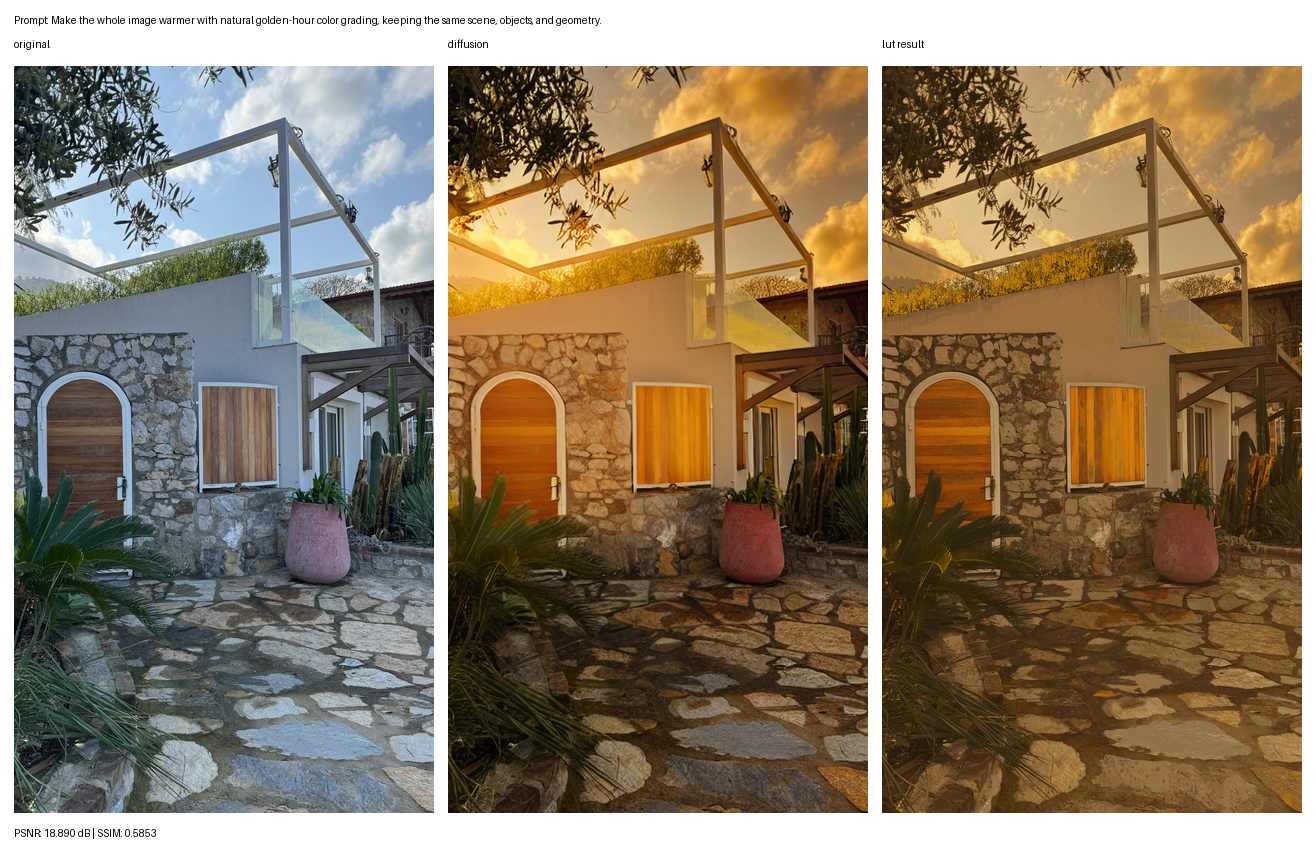
\includegraphics[width=0.8\textwidth]{immagini/house/house_golden_comp.png}
    \caption{House: comparison prodotta con il prompt ``Make the whole image warmer with natural golden-hour color grading, keeping the same scene, objects, and geometry''.}
    \label{fig:comparison-script-house-gh}
\end{figure}

Nel caso della casa in Figura~\ref{fig:comparison-script-house-gh}, la target prodotta dal modello introduce una colorazione calda in stile golden hour, ma allo stesso tempo disturba alcuni dettagli fini. Le venature del legno vengono rese piu' uniformi e alcuni bordi della porta risultano meno precisi rispetto all'originale. Il risultato LUT, invece, trasferisce buona parte della dominante calda mantenendo la geometria della foto sorgente. Questo e' un caso favorevole per il metodo: la target fornisce una trasformazione cromatica abbastanza leggibile e la LUT permette di evitare parte delle deformazioni introdotte dal modello generativo.

\begin{figure}[H]
    \centering
    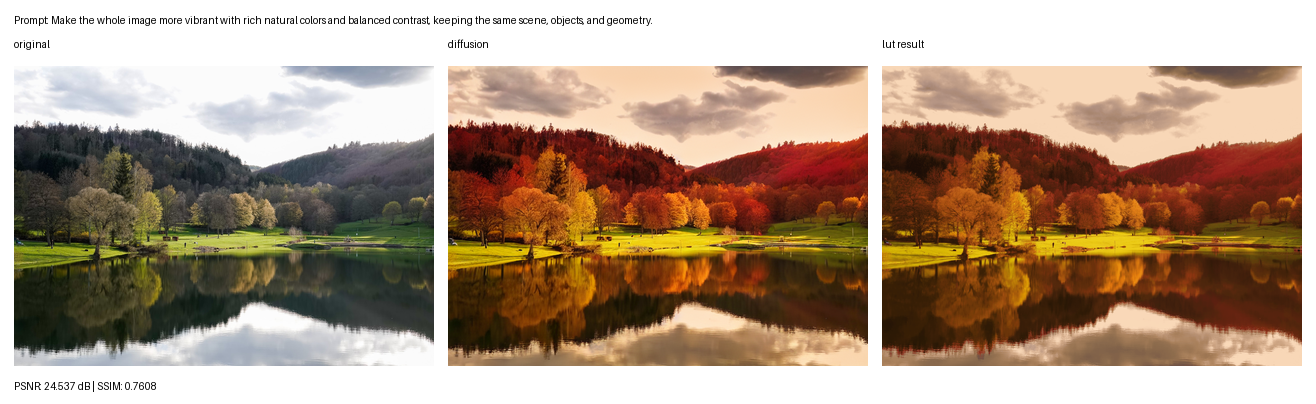
\includegraphics[width=0.8\textwidth]{immagini/lake/lake_prompt3_comparison.png}
    \caption{Lake: comparison prodotta con il prompt ``Make the whole image more vibrant with rich natural colors and balanced contrast, keeping the same scene, objects, and geometry''.}
    \label{fig:comparison-script-lake-vb}
\end{figure}

Un altro caso positivo e' quello del lago in Figura~\ref{fig:comparison-script-lake-vb}. Il prompt richiede colori naturali piu' ricchi e un contrasto bilanciato; il diffusion model modifica solo piccoli dettagli nello sfondo e mantiene sostanzialmente stabile la struttura della scena. La LUT funziona bene perche' il cambiamento richiesto e' principalmente cromatico: il risultato finale appare piu' vibrante, ma conserva la disposizione degli elementi dell'immagine originale.

\begin{figure}[H]
    \centering
    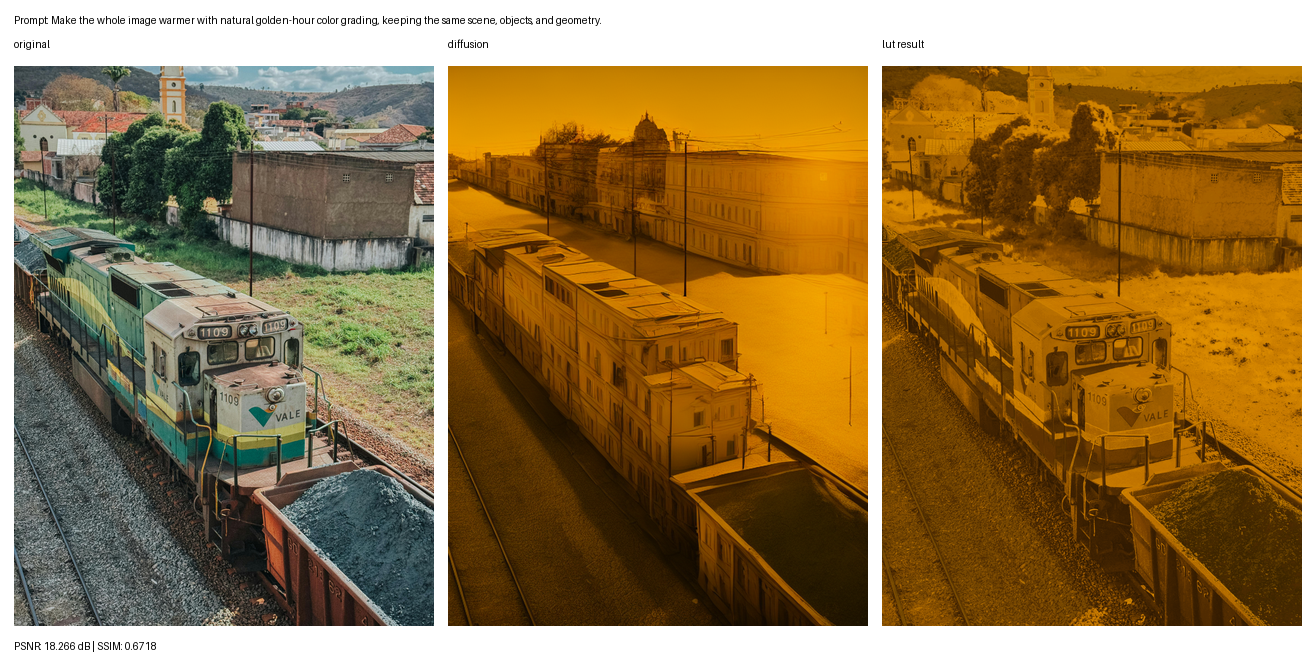
\includegraphics[width=0.8\textwidth]{immagini/train/train_prompt1_comparison.png}
    \caption{Train: comparison prodotta con il prompt ``Make the whole image more vibrant with rich natural colors and balanced contrast, keeping the same scene, objects, and geometry''.}
    \label{fig:comparison-script-train-gh}
\end{figure}

Il caso del treno in Figura~\ref{fig:comparison-script-train-gh} e' piu' ambiguo. Il risultato LUT e' visivamente gradevole, ma la target generata dal modello contiene gia' un errore importante: il soggetto principale viene rigenerato in modo non fedele e alcune parti del treno sembrano assumere l'aspetto di un edificio. Questo mostra un limite della valutazione basata solo sulla somiglianza alla target: la LUT non deve necessariamente imitare una target geometricamente sbagliata. In questo caso il risultato LUT e' utile proprio perche' mantiene la struttura dell'originale, ma il fitting risulta meno preciso perche' le coppie pixel-wise non descrivono piu' esattamente lo stesso contenuto.\newline


Quando la target generata dal modello non contiene una trasformazione cromatica chiara, anche la LUT risultante diventa poco significativa. Questo succede soprattutto con prompt che richiedono un raffreddamento marcato dell'immagine, ad esempio ``Make the whole image cooler with realistic blue cinematic color grading, keeping the same scene, objects, and geometry''. In questi casi il modello tende a produrre una target piatta, con una dominante fredda molto uniforme e poco legata ai materiali della scena.

\begin{figure}[H]
    \centering
    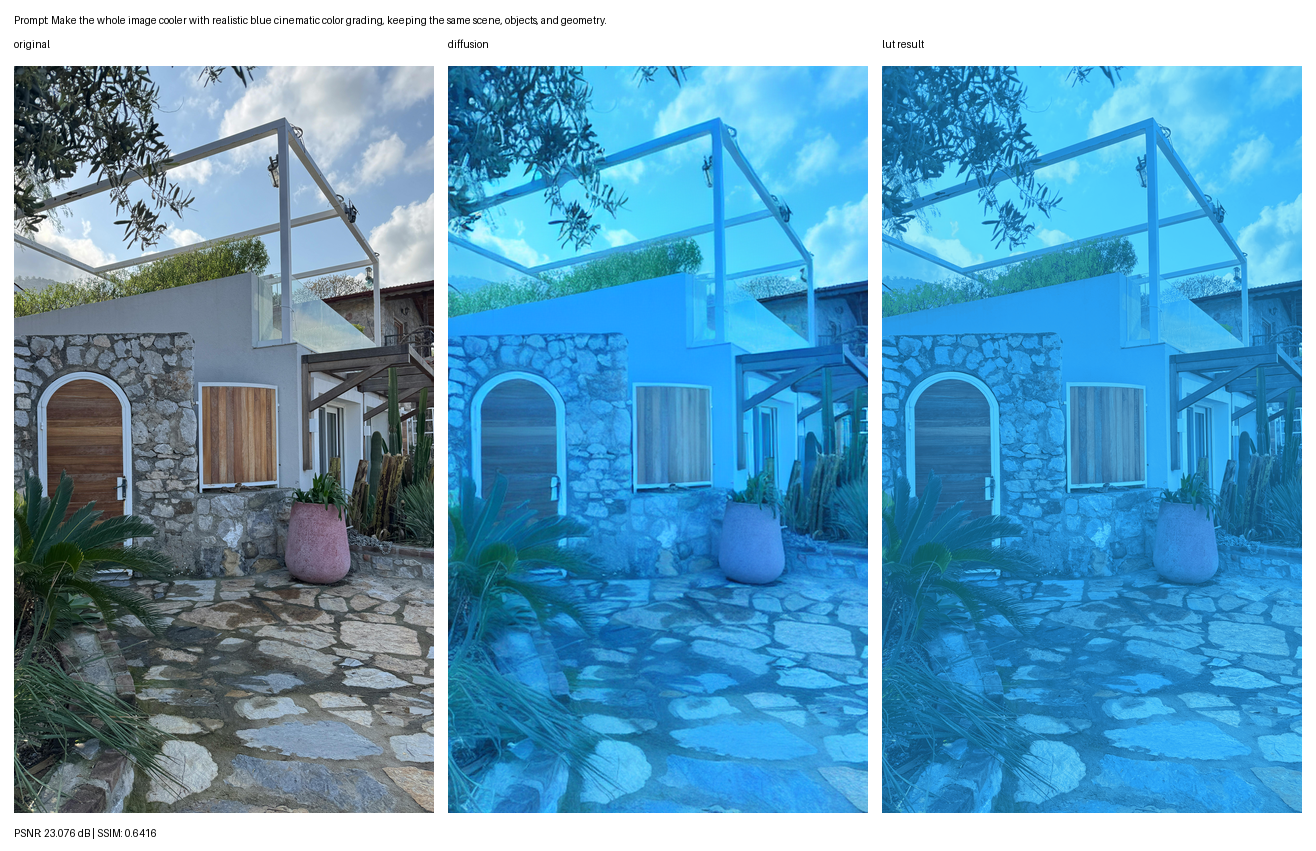
\includegraphics[width=0.8\textwidth]{immagini/house/house_prompt2_comparison.png}
    \caption{House: comparison prodotta con il prompt ``Make the whole image cooler with realistic blue cinematic color grading, keeping the same scene, objects, and geometry''.}
    \label{fig:comparison-script-house-b}
\end{figure}

In Figura~\ref{fig:comparison-script-house-b} la target non fornisce una trasformazione cromatica stabile da apprendere. Il modello raffredda l'immagine in modo uniforme e non conserva bene la separazione tra pietra, vegetazione, cielo e superfici architettoniche. Di conseguenza la LUT non riesce a trovare una mappatura colore ricca, ma produce un risultato che appare come una patina azzurra applicata sopra la fotografia originale. Questo esempio mostra che la LUT non puo' compensare una target poco informativa: se il modello generativo produce un riferimento debole, il fitting apprende una trasformazione media altrettanto debole.

\section{Stable Diffusion img2img}

Con il backend \texttt{img2img} sono stati usati parametri piu' aggressivi rispetto a InstructPix2Pix, in particolare \texttt{strength} pari a 0.45 e guidance scale pari a 9.0. Questo permette al modello di produrre target cromaticamente piu' marcate, ma aumenta anche la probabilita' che vengano modificati dettagli locali, texture e illuminazione. I due esempi seguenti mostrano bene questo trade-off.

\begin{figure}[H]
    \centering
    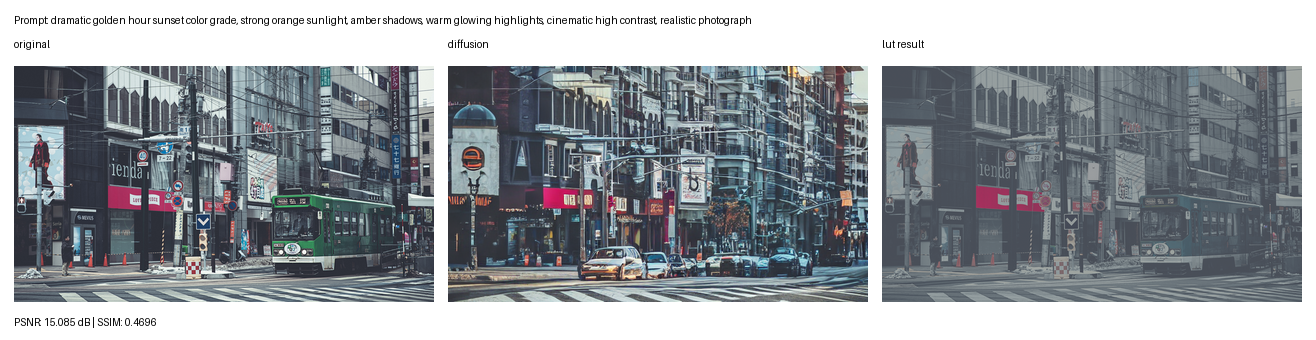
\includegraphics[width=0.9\textwidth]{immagini/img2img/city_tram_prompt1_comparison.png}
    \caption{City-tram con backend \texttt{img2img}. Il modello produce una target molto diversa localmente; la LUT conserva la struttura originale ma non riesce a riprodurre le variazioni spaziali della target.}
    \label{fig:img2img-city-tram}
\end{figure}

Nel caso della citta' in Figura~\ref{fig:img2img-city-tram}, il problema non e' solo una variazione di contrasto o atmosfera. La target modifica proprio la geometria della scena: alcune parti della strada sembrano incollate in punti non coerenti, il tram viene eliminato e la composizione non corrisponde piu' all'immagine originale. In questa situazione il fitting della LUT perde significato, perche' il pixel dell'originale e il pixel corrispondente nella target non rappresentano piu' lo stesso punto della scena. Il risultato LUT mantiene linee, tram, edifici e segnaletica dell'originale, ma non puo' imitare una target che ha cambiato soggetti e struttura. Le metriche sono infatti basse, con PSNR 15.08 dB e SSIM 0.470: non indicano soltanto una differenza cromatica, ma soprattutto una mancata corrispondenza geometrica.

\begin{figure}[H]
    \centering
    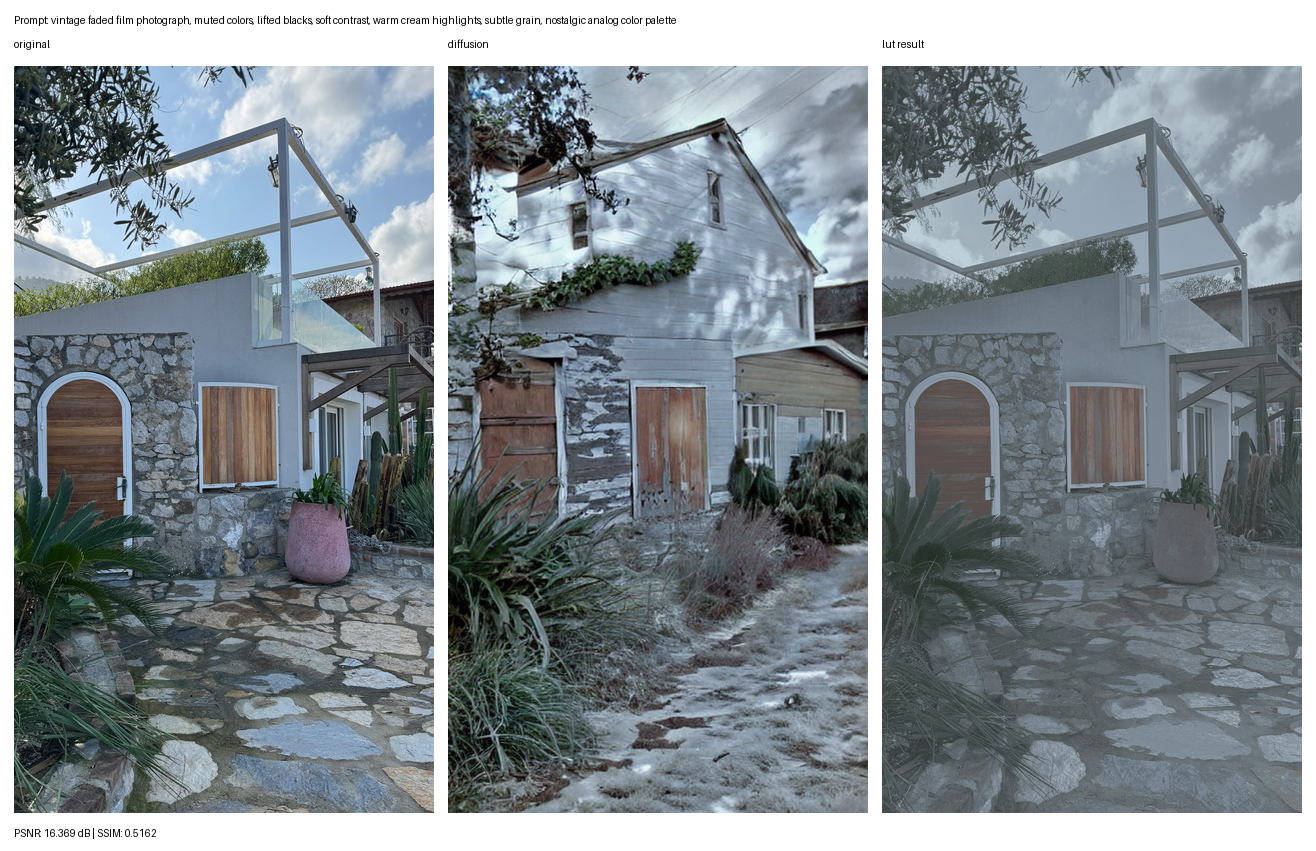
\includegraphics[width=0.8\textwidth]{immagini/img2img/house_prompt4_comparison.png}
    \caption{House con backend \texttt{img2img}. La target modifica la struttura della scena, aggiungendo elementi e cambiando parti dell'edificio, rendendo il fitting della LUT poco affidabile.}
    \label{fig:img2img-house}
\end{figure}

Anche nell'esempio della casa in Figura~\ref{fig:img2img-house} il problema principale non e' una semplice trasformazione cromatica non uniforme. La target modifica in modo sostanziale la scena: aggiunge cespugli e vegetazione, cambia la casa sullo sfondo, altera il cielo e modifica anche la strada. In questo modo la target non rappresenta piu' la stessa immagine ricolorata, ma una scena parzialmente rigenerata. La LUT, che puo' apprendere solo una mappatura RGB globale, riceve quindi corrispondenze pixel-wise sbagliate: pixel che nell'originale appartengono a pietra, muro o strada vengono confrontati con pixel che nella target appartengono a elementi nuovi o modificati. Il risultato finale diventa quindi molto debole e visivamente sporco, perche' la LUT prova a mediare trasformazioni che non hanno una relazione cromatica coerente. Il valore PSNR 16.37 dB e SSIM 0.516 conferma che la distanza dalla target non e' dovuta solo al colore, ma soprattutto al cambio di contenuto e geometria.

\section{SDXL Turbo}

Il backend \texttt{sdxl-turbo} e' stato testato per valutare un modello piu' rapido, capace di generare una target in pochi step. In questo esperimento, pero', la velocita' va a scapito della coerenza dell'immagine generata. La target non risulta semplicemente diversa dall'originale: diventa logicamente e fisicamente poco riconoscibile, con artefatti grafici evidenti.

\begin{figure}[H]
    \centering
    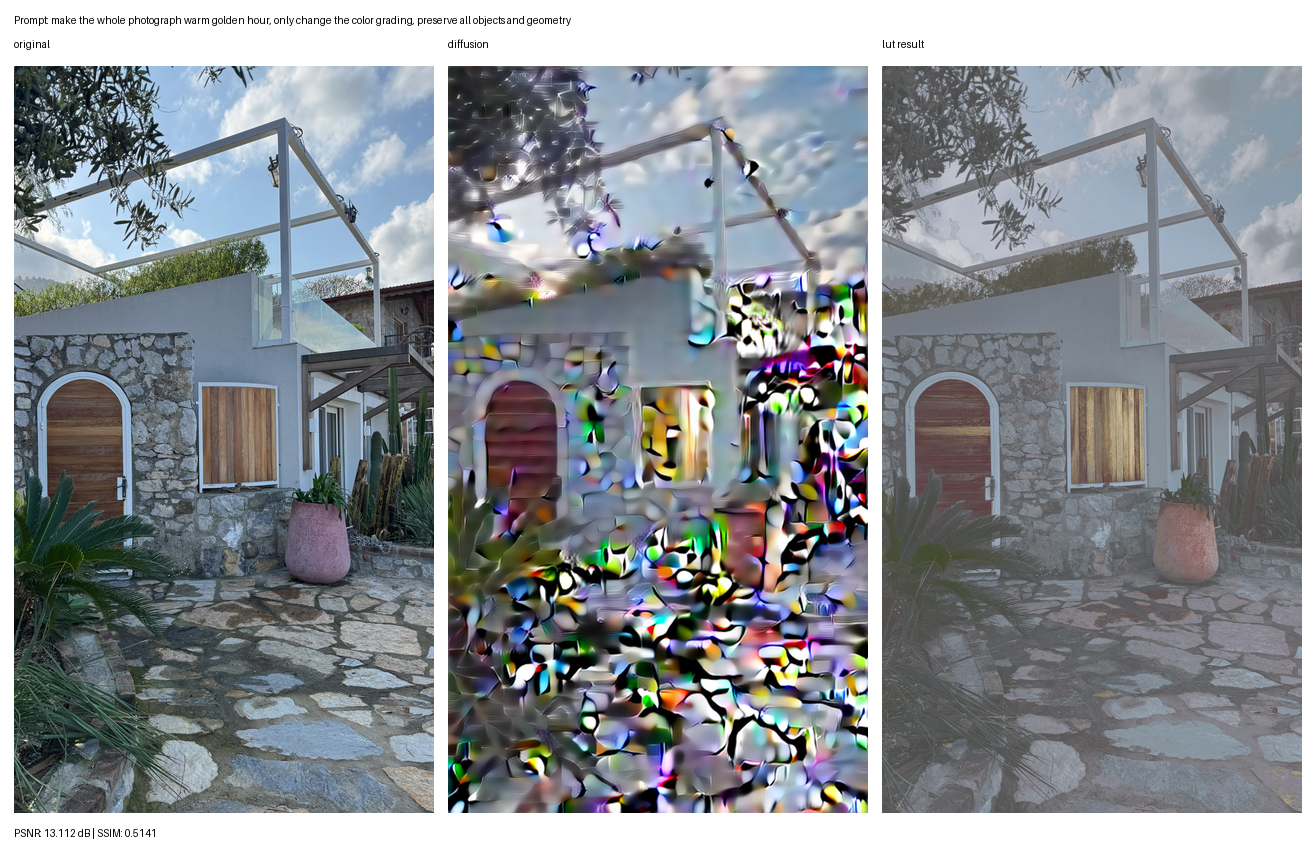
\includegraphics[width=0.8\textwidth]{immagini/sdxl_turbo/house_sdxl_turbo_comparison.png}
    \caption{House con backend \texttt{sdxl-turbo}. La target presenta artefatti grafici e una struttura fisica irriconoscibile, rendendo il fitting della LUT poco significativo.}
    \label{fig:sdxl-turbo-house}
\end{figure}

In Figura~\ref{fig:sdxl-turbo-house} quello che nell'originale era una casa viene trasformato in una massa di pixel luminosi e poco interpretabili. La target non conserva in modo affidabile pareti, porta, pietre, vegetazione e profondita' della scena; non e' quindi una semplice ricolorazione calda o contrastata, ma un fallimento logico della generazione. In queste condizioni la LUT non puo' funzionare come previsto, perche' non esiste una trasformazione colore coerente da apprendere. Il risultato LUT conserva la geometria della foto sorgente, ma appare lontano dalla target perche' la target stessa non e' piu' fisicamente comparabile all'originale. Le metriche sono tra le piu' basse osservate, con PSNR 13.11 dB e SSIM 0.514, e vanno interpretate come segnale di fallimento del target generativo, non come difetto del formato LUT.

\section{Risultati Gemini e refinement residual}

I risultati ottenuti con Gemini (Nanobanana) sono interessanti perche' il modello produce target visivamente piu' curate e spesso piu' stabili nella geometria globale. Tuttavia, anche quando la scena sembra preservata, il modello puo' aggiungere dettagli locali (come modificare cartelli o scritte), luci, riflessi e variazioni di ombra non presenti nell'originale. Questo e' il caso in cui il limite della LUT globale diventa piu' evidente: il risultato non fallisce perche' la target e' brutta, ma perche' la target e' troppo ricca localmente per essere approssimata con una sola funzione RGB.

\begin{figure}[H]
    \centering
    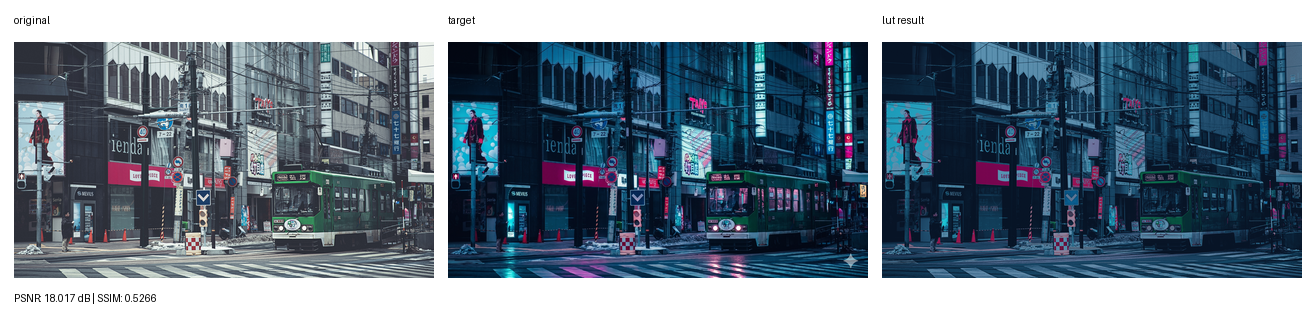
\includegraphics[width=\textwidth]{immagini/gemini/city_tram_gemini_lut_comparison.png}
    \caption{City-tram con target Gemini e sola LUT globale. La target introduce luci neon e riflessi locali che la LUT non riesce a trasferire selettivamente.}
    \label{fig:gemini-city-tram-lut}
\end{figure}

Nel caso \texttt{city-tram}, mostrato in Figura~\ref{fig:gemini-city-tram-lut}, Gemini mantiene riconoscibile la scena ma la trasforma in una versione notturna con luci cyan e magenta. I riflessi sull'asfalto e le insegne illuminate sono pero' effetti spaziali: non dipendono solo dal colore originale del pixel, ma dalla posizione e dal contenuto della scena. La LUT globale non puo' distinguere due pixel grigi simili se uno nella target diventa riflesso neon e l'altro rimane scuro. Il risultato e' quindi una dominante blu complessiva, con PSNR 18.02 dB e SSIM 0.527.

\begin{figure}[H]
    \centering
    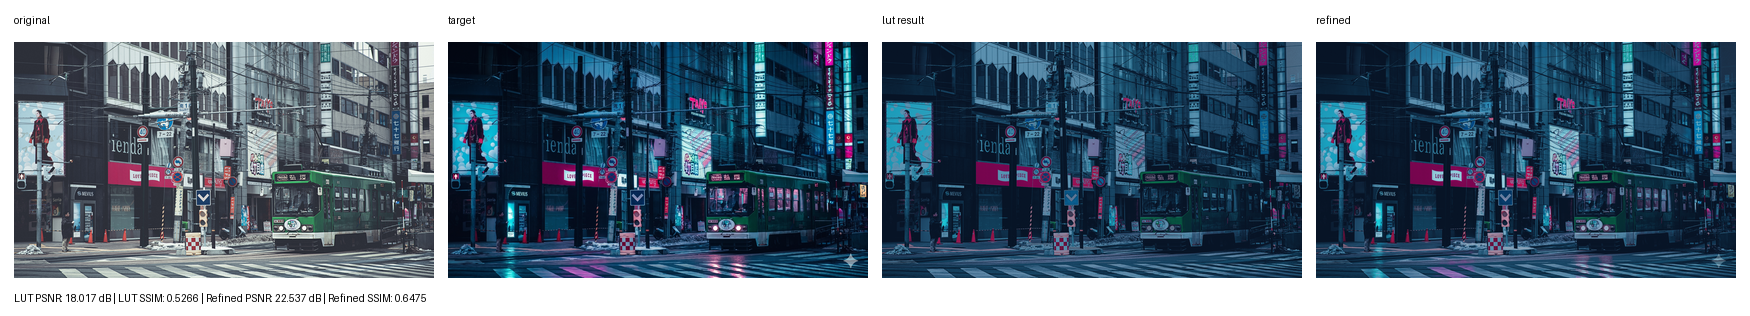
\includegraphics[width=\textwidth]{immagini/gemini/city_tram_gemini_refined_comparison.png}
    \caption{City-tram con refinement residual. Il quarto pannello mostra il recupero parziale di riflessi e accensioni locali rispetto alla sola LUT.}
    \label{fig:gemini-city-tram-refined}
\end{figure}

Applicando il refinement residual, come in Figura~\ref{fig:gemini-city-tram-refined}, il risultato si avvicina maggiormente alla target: PSNR e SSIM passano rispettivamente a 22.54 dB e 0.648. Il miglioramento e' visibile soprattutto nei riflessi e nelle zone piu' luminose, ma resta un compromesso. Se il residual viene applicato troppo, si rischia di importare direttamente dettagli generati; se viene applicato poco, il risultato torna a essere una LUT globale con effetto filtro.

\begin{figure}[H]
    \centering
    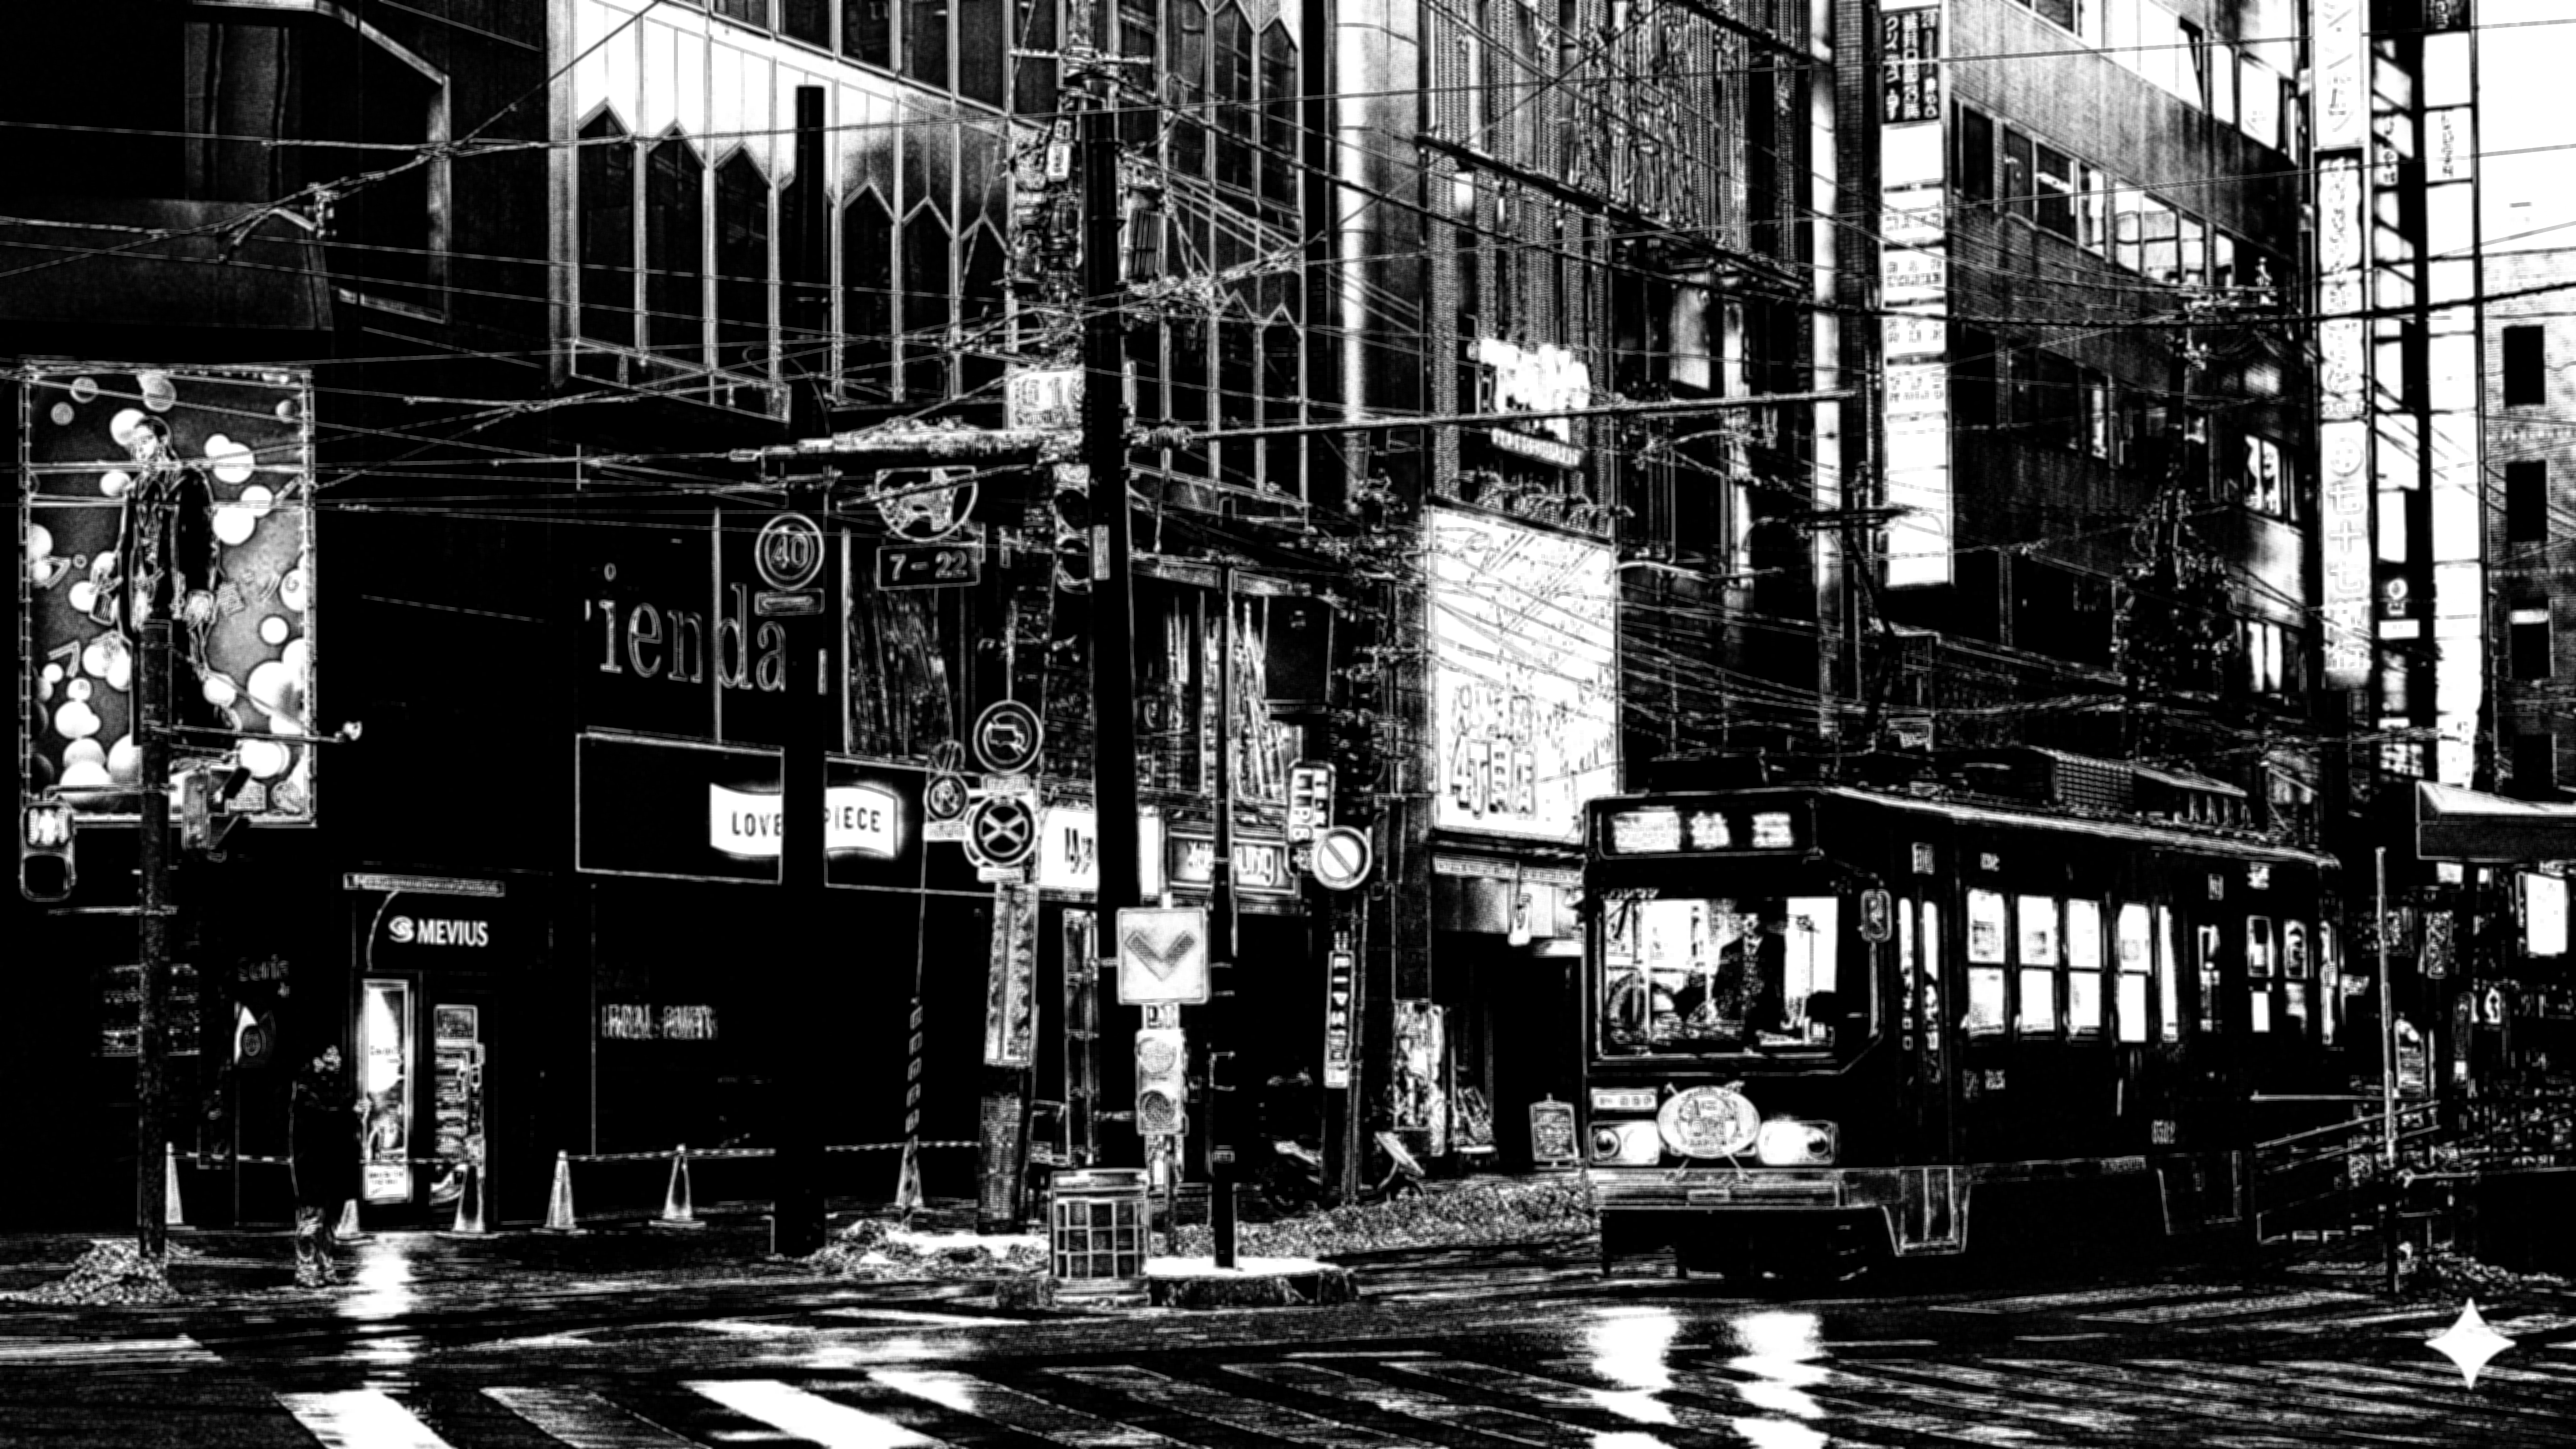
\includegraphics[height=7cm]{immagini/gemini/city_tram_gemini_refined_mask.png}
    \caption{Maschera residual per il caso city-tram. Le zone piu' chiare indicano dove il refinement applica piu' correzione locale.}
    \label{fig:gemini-city-tram-mask}
\end{figure}

\begin{figure}[H]
    \centering
    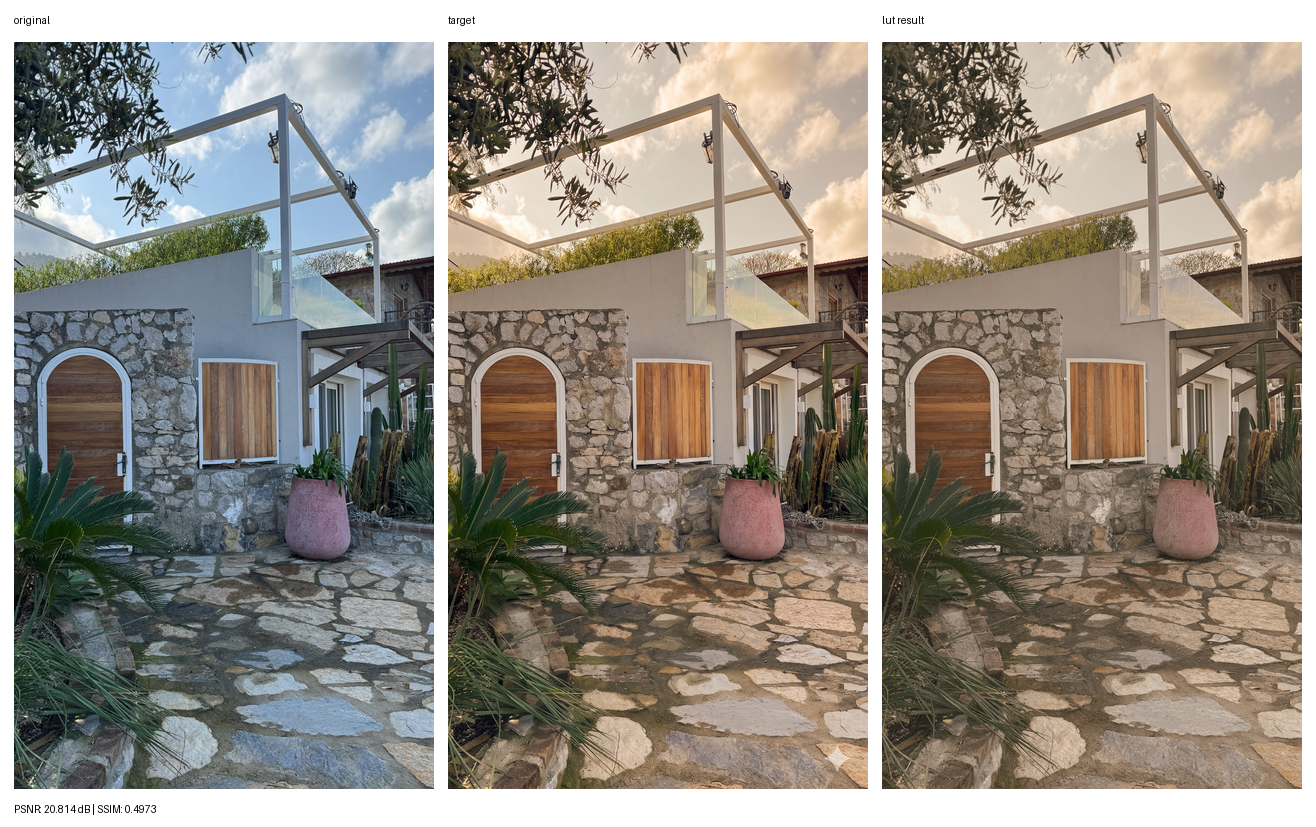
\includegraphics[width=0.9\textwidth]{immagini/gemini/house_gemini_lut_comparison.png}
    \caption{House con target Gemini e sola LUT globale. Il risultato e' credibile come filtro caldo, ma perde parte delle variazioni locali della target.}
    \label{fig:gemini-house-lut}
\end{figure}

Il caso \texttt{house}, riportato in Figura~\ref{fig:gemini-house-lut}, e' meno estremo. La target Gemini produce una colorazione calda e abbastanza coerente, ma modifica comunque il cielo, le ombre, la vegetazione e alcune luci locali. La sola LUT porta l'immagine verso la dominante dorata, ma appiattisce le differenze spaziali e non recupera completamente la luminosita' della target. Le metriche della LUT sono PSNR 20.81 dB e SSIM 0.497.

\begin{figure}[H]
    \centering
    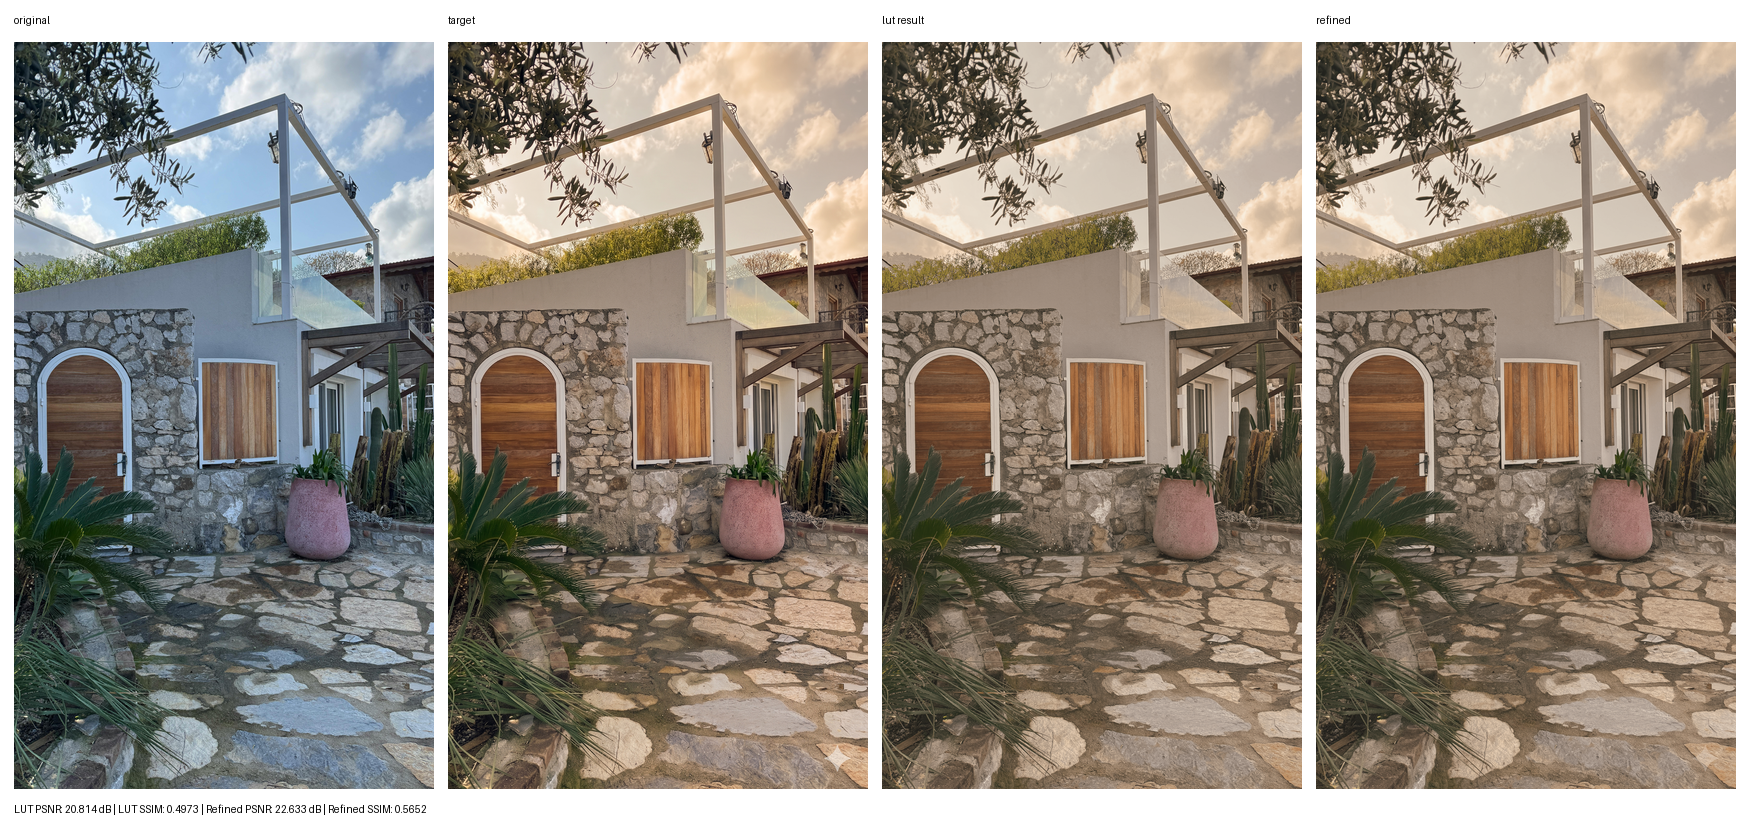
\includegraphics[width=0.9\textwidth]{immagini/gemini/house_gemini_refined_comparison.png}
    \caption{House con refinement residual. Il refined recupera parte della luminosita' e delle variazioni locali introdotte dalla target.}
    \label{fig:gemini-house-refined}
\end{figure}

Con il refinement, visibile in Figura~\ref{fig:gemini-house-refined}, il risultato migliora a PSNR 22.63 dB e SSIM 0.565. Anche qui il vantaggio principale e' il recupero di componenti locali che la LUT non puo' modellare. Il risultato non deve pero' essere interpretato come sostituto della LUT: e' una fase aggiuntiva che sacrifica parte della purezza della trasformazione globale per avvicinarsi alla target generativa.




\section{Limiti della LUT globale}

La 3D LUT stimata nel progetto rappresenta una trasformazione definita nello spazio RGB: a colori sorgente simili vengono associate trasformazioni simili, indipendentemente dalla posizione del pixel e dal contenuto semantico della scena. Questa proprieta' rende la LUT adatta a trasferire un color grading globale, ma ne limita l'efficacia quando la target generata dal diffusion model contiene variazioni spaziali non riconducibili al solo colore.

Il fitting e' quindi ben posto solo se la target conserva una corrispondenza pixel-wise sufficientemente stabile con l'immagine originale. Quando il modello modifica oggetti, geometria, prospettiva, scritte, texture, ombre o riflessi locali, le coppie source-target non descrivono piu' una trasformazione cromatica coerente. In questi casi la LUT approssima una media tra corrispondenze incompatibili: il risultato preserva la geometria originale, ma il trasferimento cromatico tende ad apparire come una correzione globale poco selettiva.

L'implementazione usa interpolazione trilineare nella griglia RGB, una scelta comune per l'applicazione di LUT 3D; OpenColorIO descrive l'interpolazione lineare su \textit{Lut3D} come trilineare \cite{opencolorio_interpolation}. Il formato \texttt{.cube} salvato dal progetto segue la struttura tipica con dichiarazione \texttt{LUT\_3D\_SIZE} e triplette RGB \cite{cube_format}. I limiti osservati dipendono quindi principalmente dalla qualita' e dall'allineamento della target generativa, non dal formato della LUT \cite{brooks_instructpix2pix}.

\chapter{Conclusioni}

I test mostrano che l'uso di una 3D LUT e' efficace quando la target generata dal diffusion model rappresenta principalmente una ricolorazione dell'immagine originale. In questi casi la LUT permette di trasferire il color grading desiderato mantenendo la geometria della sorgente e riducendo alcuni artefatti introdotti dal modello generativo. Negli esempi con InstructPix2Pix, la casa con colorazione \textit{golden hour} e il paesaggio del lago mostrano questo comportamento: la target fornisce una direzione cromatica leggibile, mentre il risultato LUT conserva meglio bordi, texture e struttura dell'immagine originale. Lo stesso principio e' utile quando il modello altera piccoli dettagli, ad esempio scritte, insegne o elementi fini: la LUT non copia direttamente tali modifiche, ma applica solo la trasformazione cromatica appresa.

Il limite principale emerge quando gli artefatti del diffusion model non sono piccoli errori locali, ma modifiche sostanziali della scena. Negli esperimenti con \texttt{img2img}, ad esempio, la target della citta' elimina il tram e modifica parti della strada, mentre la target della casa aggiunge vegetazione, cambia il cielo, la strada e parti dell'edificio. In questi casi la LUT non dispone piu' di coppie pixel-wise coerenti da cui apprendere: prova quindi a mediare trasformazioni incompatibili e il risultato finale assume l'aspetto di un filtro cromatico raffazzonato, lontano dalla ricolorazione richiesta nella pipeline completa. Il caso \texttt{sdxl-turbo} e' ancora piu' evidente, perche' la target degrada fisicamente il soggetto e rende impossibile stimare una trasformazione colore significativa.

Gli esperimenti indicano inoltre che il risultato dipende in modo forte dal modello utilizzato e dal prompt. InstructPix2Pix si e' dimostrato piu' adatto alla semplice ricolorazione rispetto al backend \texttt{img2img} con parametri piu' aggressivi, perche' tende a preservare meglio la struttura della scena. Anche all'interno dello stesso backend, prompt piu' vincolati alla conservazione di scena, oggetti e geometria producono target piu' utili per il fitting, mentre prompt troppo generici o troppo marcati aumentano il rischio di alterazioni non cromatiche.

Una limitazione sperimentale e' stata l'esecuzione locale dei modelli, che ha imposto l'uso di backend e parametri compatibili con le risorse disponibili. I risultati ottenuti con target prodotte da modelli piu' capaci, come Gemini, mostrano che una target generativa piu' stabile puo' migliorare sensibilmente la qualita' finale. Rimane pero' aperta una questione metodologica: se la capacita' dei modelli image-to-image cresce abbastanza da produrre direttamente ricolorazioni fedeli, coerenti e prive di artefatti geometrici, diventa necessario valutare se l'uso intermedio di una 3D LUT sia ancora vantaggioso oppure se resti utile solo come vincolo deterministico per preservare l'immagine originale.

\begin{thebibliography}{9}

\bibitem{opencolorio_interpolation}
Academy Software Foundation.
\textit{OpenColorIO documentation: Interpolation enum}.
Disponibile online: \texttt{https://opencolorio.readthedocs.io/en/v2.4.1/api/enums.html}.

\bibitem{cube_format}
TwineConvert.
\textit{CUBE (Adobe CUBE LUT) format guide}.
Disponibile online: \texttt{https://twineconvert.com/formats/cube}.

\bibitem{brooks_instructpix2pix}
T. Brooks, A. Holynski, A. A. Efros.
\textit{InstructPix2Pix: Learning to Follow Image Editing Instructions}.
CVPR 2023. Disponibile online: \texttt{https://arxiv.org/abs/2211.09800}.

\end{thebibliography}

\end{document}
